\section{Proxy construction framework}
\label{sec:framework}

\subsection{Role of proxies in emission downscaling}

Spatial proxies define how emissions reported on a coarse inventory grid
are redistributed to the finer grid required by urban air-quality
modelling. They are therefore not auxiliary cartographic products, but
the main methodological link between an emission inventory and the
spatial pattern imposed on the downscaled emissions. For each pollutant
and sector, the proxy must represent the location of the activity that
generates the emissions as closely as the available evidence allows.

This requirement is particularly important for \cams, because emissions
are reported by GNFR sector and by pollutant, while the spatial drivers
of the processes grouped inside one GNFR sector may differ substantially.
A single land-cover mask can be adequate for a homogeneous residual
source, but it is not sufficient when a sector contains point facilities,
linear infrastructure, population-related activities, industrial land,
livestock processes, or fuel-specific combustion patterns. The proxy
methodology was therefore redesigned around the principle that the
spatialisation method must follow the emission process rather than the
sector label alone.
\begin{figure}[htbp]
  \centering
  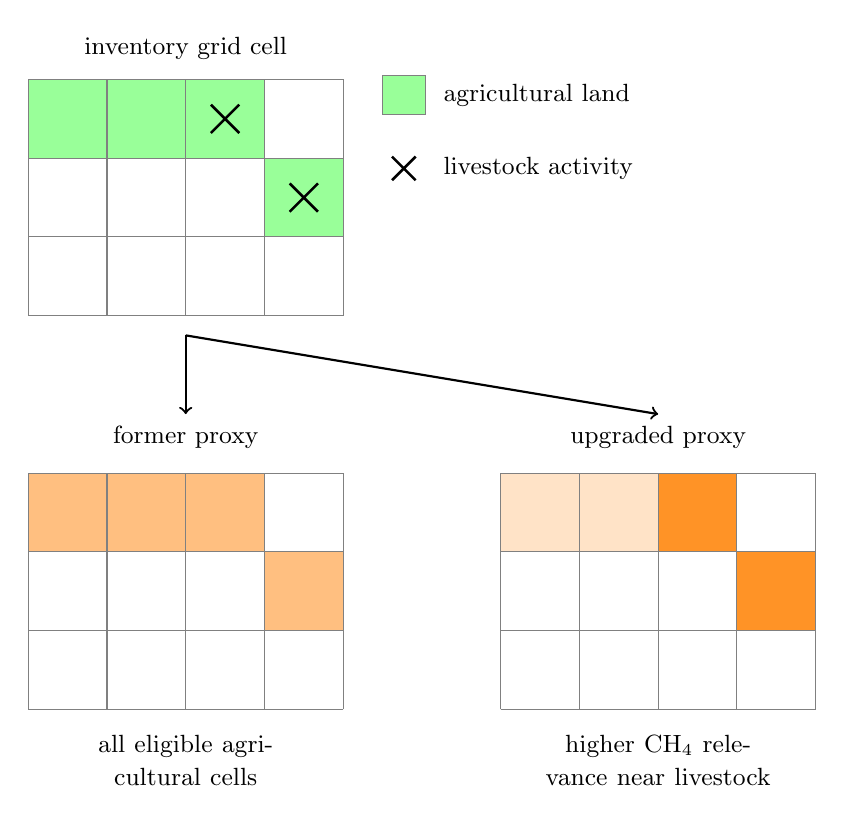
\begin{tikzpicture}[x=1cm, y=1cm]

    %% =========================================================
    %% TOP GRID — bottom-left (0,0), top-right (4,3)
    %% Row 2 (top row):    y = 2 to 3
    %% Row 1 (middle row): y = 1 to 2
    %% Row 0 (bottom row): y = 0 to 1
    %% =========================================================
    \node[align=center] at (2.0, 3.4) {\small inventory grid cell};

    \fill[green!40] (0,2) rectangle (1,3);
    \fill[green!40] (1,2) rectangle (2,3);
    \fill[green!40] (2,2) rectangle (3,3);
    \fill[green!40] (3,1) rectangle (4,2);

    \draw[step=1, line width=0.4pt, color=black!50] (0,0) grid (4,3);

    \foreach \cx/\cy in {2.5/2.5, 3.5/1.5}{
      \draw[line width=0.9pt]
        (\cx-0.18,\cy-0.18)--(\cx+0.18,\cy+0.18)
        (\cx-0.18,\cy+0.18)--(\cx+0.18,\cy-0.18);
    }

    %% LEGEND
    \fill[green!40]   (4.5,2.55) rectangle (5.05,3.05);
    \draw[black!50, line width=0.4pt] (4.5,2.55) rectangle (5.05,3.05);
    \node[anchor=west] at (5.15,2.80) {\small agricultural land};
    \draw[line width=0.9pt]
      (4.62,1.72)--(4.92,2.02)
      (4.62,2.02)--(4.92,1.72);
    \node[anchor=west] at (5.15,1.87) {\small livestock activity};

    %% ARROWS
    \draw[->, line width=0.8pt] (2.0,-0.25) -- (2.0,-1.25);
    \draw[->, line width=0.8pt] (2.0,-0.25) -- (8.0,-1.25);

    %% =========================================================
    %% BOTTOM-LEFT: former proxy
    %% Grid bottom-left (0,-5), top-right (4,-2)
    %% So 3 rows:
    %%   top row    (row2): y = -3 to -2
    %%   middle row (row1): y = -4 to -3
    %%   bottom row (row0): y = -5 to -4
    %%
    %% Pattern mirrors top grid:
    %%   col0,col1,col2 in top row    => y=-3 to -2
    %%   col3           in middle row => y=-4 to -3
    %% =========================================================
    \node[align=center] at (2.0,-1.55) {\small former proxy};

    % TOP ROW fills: y from -3 to -2
    \fill[orange!50] (0,-3) rectangle (1,-2);
    \fill[orange!50] (1,-3) rectangle (2,-2);
    \fill[orange!50] (2,-3) rectangle (3,-2);
    % MIDDLE ROW fill: y from -4 to -3
    \fill[orange!50] (3,-4) rectangle (4,-3);

    \draw[step=1, line width=0.4pt, color=black!50] (0,-5) grid (4,-2);

    \node[align=center, text width=3.0cm] at (2.0,-5.65)
      {\small all eligible agricultural cells};

    %% =========================================================
    %% BOTTOM-RIGHT: upgraded proxy
    %% Grid bottom-left (6,-5), top-right (10,-2)
    %% Same cell positions, differentiated intensity:
    %%   col0,col1 in top row    => LOW  intensity
    %%   col2      in top row    => HIGH intensity
    %%   col3      in middle row => HIGH intensity
    %% =========================================================
    \node[align=center] at (8.0,-1.55) {\small upgraded proxy};

    % TOP ROW
    \fill[orange!22] (6,-3)  rectangle (7,-2);   % col0 low
    \fill[orange!22] (7,-3)  rectangle (8,-2);   % col1 low
    \fill[orange!85] (8,-3)  rectangle (9,-2);   % col2 HIGH
    % MIDDLE ROW
    \fill[orange!85] (9,-4)  rectangle (10,-3);  % col3 HIGH

    \draw[step=1, line width=0.4pt, color=black!50] (6,-5) grid (10,-2);

    \node[align=center, text width=3.5cm] at (8.0,-5.65)
      {\small higher CH$_4$ relevance near livestock};

  \end{tikzpicture}
  \caption{Simplified motivation for process-specific proxy construction.
    A broad agricultural land-cover proxy spreads emissions uniformly over
    all eligible agricultural cells, whereas a process-specific proxy
    amplifies CH$_4$ relevance where livestock activity is present.}
  \label{fig:proxy-process-motivation}
\end{figure}





\subsection{From the former workflow to the upgraded methodology}

The previous UrbEm proxy workflow already provided an operational basis
for downscaling. It constructed a regular modelling grid, prepared
population and land-cover rasters, used selected infrastructure and
facility layers, and produced a set of sectoral proxy rasters. This
former implementation was reviewed sector by sector before the upgrade.
The objective was not to discard the existing methodology, but to
identify which assumptions remained appropriate, which ones were too
generic, and where the treatment of point and area emissions needed to
be separated more explicitly.

The review showed three main limitations. First, several sectors were
represented by broad composite land-cover layers, which made all
pollutants within the same sector inherit the same spatial pattern.
Second, point-like industrial or infrastructure sources were not always
distinguished from residual area sources in a transparent way. Third,
the former procedure was difficult to audit because data preparation,
sector logic, fallback assumptions, and output generation were combined
in a single procedural workflow. These limitations are acceptable for a
first proxy inventory, but they become restrictive when the objective is
to produce sector-specific, pollutant-aware, and reproducible
downscaling weights.

The upgraded methodology therefore separates the proxy problem into
explicit methodological components. Point-source emissions are treated
through a dedicated matching procedure between inventory points and
external facility datasets. Area-source emissions are treated through
sector-specific proxy construction, ranging from simple robust proxies
to multi-dataset and process-specific combinations. This structure makes
the assumptions attached to each sector visible and allows the proxy
outputs to better reflect the heterogeneity of the CAMS emission
structure.

\begin{figure}[htbp]
  \centering
  \setlength{\fboxsep}{5pt}
  \begin{tabular}{c c c c c}
    \fbox{\begin{minipage}{0.17\textwidth}\centering
      Legacy proxy\\workflow
    \end{minipage}} &
    $\longrightarrow$ &
    \fbox{\begin{minipage}{0.20\textwidth}\centering
      Sector-by-sector\\method review
    \end{minipage}} &
    $\longrightarrow$ &
    \fbox{\begin{minipage}{0.24\textwidth}\centering
      Upgraded modular\\proxy methodology
    \end{minipage}} \\
    & & $\downarrow$ & & $\downarrow$ \\
    & &
    \fbox{\begin{minipage}{0.20\textwidth}\centering
      Identification of\\limitations and\\fallbacks
    \end{minipage}} &
    $\longrightarrow$ &
    \fbox{\begin{minipage}{0.24\textwidth}\centering
      Separate treatment of\\point and area\\emissions
    \end{minipage}}
  \end{tabular}
  \caption{Conceptual transition from the former proxy workflow to the upgraded methodology.}
  \label{fig:proxy-old-new-transition}
\end{figure}

\subsection{Point and area emissions in CAMS}

CAMS distinguishes between emissions represented as point sources and
emissions represented as area sources. This distinction is central for
proxy construction. A point source is associated with an explicit
location in the inventory and should, when possible, be linked to a real
facility or installation. An area source represents emissions that are
not resolved as individual facilities in the inventory and must be
redistributed within each CAMS grid cell using spatial indicators.

The methodological consequence is that the same GNFR sector can require
two different proxy treatments. Public power, industry, waste, and
solvent-related activities may contain point-like facilities that should
not be blurred into a generic land-use surface. At the same time, the
same sectors can retain a residual area component that must still be
distributed spatially. Other sectors, such as shipping, fugitive
emissions, off-road transport, agriculture, and residential or commercial
combustion, are dominated by area-source logic or by process-specific
spatial drivers.

\begin{figure}[htbp]
  \centering
  \includegraphics[width=0.98\textwidth]{figures/Proxies/greece_cams_area_share_heatmap.png}
  \caption{Mass share of area and point sources by GNFR sector and pollutant in the CAMS-REG v8.1 inventory for Greece (2019). The full numerical table is given in Appendix~\ref{tab:greece_cams_emis_2019}.}
  \label{fig:gr-area-point-share}
\end{figure}

The point and area contributions are therefore used as a diagnostic step
rather than as a purely descriptive statistic. They indicate whether a
sector should be handled mainly through facility matching, through
area-source proxies, or through a mixed approach. They also help
identify cases where a residual area component is not a separate
physical process, but the part of the gridded inventory that remains
after reported point sources and inventory totals are reconciled.

\begin{figure}[htbp]
  \centering
  \setlength{\fboxsep}{5pt}
  \begin{tabular}{c c c}
    \fbox{\begin{minipage}{0.25\textwidth}\centering
      CAMS emissions\\by sector, pollutant,\\and source type
    \end{minipage}} &
    $\longrightarrow$ &
    \fbox{\begin{minipage}{0.27\textwidth}\centering
      Point-source\\matching to external\\facility records
    \end{minipage}} \\
    $\downarrow$ & & $\downarrow$ \\
    \fbox{\begin{minipage}{0.25\textwidth}\centering
      Sector-specific\\area-source proxy\\construction
    \end{minipage}} &
    $\longrightarrow$ &
    \fbox{\begin{minipage}{0.27\textwidth}\centering
      Normalised proxy\\weights and quality\\control outputs
    \end{minipage}}
  \end{tabular}
  \caption{High-level data flow of the upgraded proxy methodology.}
  \label{fig:proxy-upgraded-dataflow}
\end{figure}

\subsection{Structure of the proxy methodology}

The heatmap in Figure~\ref{fig:gr-area-point-share} shows that the
point--area split is not uniform across sectors or pollutants. Some
sectors are almost entirely area-source in CAMS and can therefore be
handled through area-weight rasters alone. Others contain large point
contributions, or pollutant-dependent mixtures of point and area
emissions, and require a separate facility-matching step before the
residual area component is distributed.

For this reason, the following sections are organised by methodological
need rather than by inventory order. Point-source matching is presented
first because it determines which emissions are assigned to explicit
facilities and should not be redistributed as diffuse area emissions.
Area-source proxies are then described according to increasing
methodological complexity: simple single-layer proxies, combined
multi-dataset proxies, and highly customised process-based approaches.
This structure avoids treating all GNFR sectors as if they required the
same spatial evidence, while keeping the chapter focused on the logic of
proxy construction rather than on a catalogue of outputs.

\subsection{General weight construction}

Although the sectoral methods differ, the area-source part of the
workflow follows a common mathematical logic. Each sector first defines
one or more non-negative spatial indicators on the target reference
grid. These indicators may represent land cover, population, facility
density, transport infrastructure, vessel activity, building-energy
demand, livestock distributions, or other sector-specific drivers. The
indicators are then combined into a raw proxy score and normalised so
that the weights inside each CAMS cell sum to unity.

\subsubsection{Notation}

Throughout this section, the following notation is used:

\begin{table}[h]
  \centering
  \caption{Core notation used for area-source proxy construction.}
  \label{tab:proxy-notation}
  \begin{tabular}{ll}
    \toprule
    Symbol & Meaning \\
    \midrule
    $p$ & pollutant \\
    $s$ & GNFR sector or sectoral component \\
    $m$ & spatial driver, process source, or subsector layer \\
    $j$ & fine-resolution target-grid cell \\
    $C$ & CAMS grid cell containing one or more target-grid cells \\
    $x_{j,m}$ & raw non-negative spatial indicator for driver $m$ in cell $j$ \\
    $\rho_{j,m}$ & scaled relevance of driver $m$ in cell $j$ \\
    $a_{p,m}$ & allocation coefficient for pollutant $p$ and driver $m$ \\
    $S_{j,p}$ & raw combined proxy score for pollutant $p$ in cell $j$ \\
    $w_{j,p}$ & final normalised proxy weight for pollutant $p$ in cell $j$ \\
    \bottomrule
  \end{tabular}
\end{table}

\subsubsection{Spatial indicators and relevance}
\label{sec:relevance-rho}

The raw indicator $x_{j,m}$ expresses the intensity or suitability of
target-grid cell $j$ for spatial driver $m$. Its definition is
sector-specific. For a land-cover proxy, it may be a binary or weighted
class mask. For an infrastructure proxy, it may be the presence or
density of a line or polygon feature. For a process-based proxy, it may
combine several layers before being passed to the final weighting step.

When the magnitude of a raw indicator is not directly comparable across
drivers, it is converted into a dimensionless relevance value. A generic
form is

\begin{equation}
\label{eq:rho-def}
  \rho_{j,m} =
  \begin{cases}
    \dfrac{x_{j,m}}{\displaystyle\max_{j' \in \Omega_m} x_{j',m}},
    & \text{if } \displaystyle\max_{j' \in \Omega_m} x_{j',m} > 0, \\
    0,
    & \text{otherwise,}
  \end{cases}
\end{equation}

where $\Omega_m$ is the spatial support over which driver $m$ is scaled.
Depending on the sector, this support may be a country, a CAMS cell, a
regional mask, or the valid domain of the input layer. The purpose of
this step is not to estimate emissions directly, but to express relative
spatial suitability on a common scale.

\subsubsection{Spatial support and rasterisation}
\label{sec:class-extent}

All area-source indicators are converted to the same target grid before
normalisation. Raster inputs are reprojected and aligned to the
reference grid, while vector inputs are rasterised using the attributes,
buffers, or class memberships defined for the sector. The result is a
set of candidate layers whose cells are spatially comparable and can be
combined without changing the CAMS inventory totals.

This rasterisation step is also where sector-specific spatial support is
defined. Some sectors use broad land-cover classes, others use explicit
infrastructure, facility polygons, vessel-density fields, or building
and population layers. The support therefore differs by sector, but the
final weights always describe how emissions are redistributed within the
CAMS cells retained for the downscaling domain.

\subsubsection{Allocation coefficients}
\label{sec:alpha}

When several drivers contribute to a sector or pollutant, allocation
coefficients determine their relative contribution to the raw proxy
score. These coefficients are denoted by $a_{p,m}$ and may represent
subsector shares, pollutant-specific source fractions, class weights, or
reported allocation factors. For a given pollutant and sectoral
component, they are defined so that the active drivers form a consistent
mixture:

\begin{equation}
  \sum_{m \in \mathcal{M}_{p}} a_{p,m} = 1,
\end{equation}

where $\mathcal{M}_{p}$ is the set of drivers used for pollutant $p$.
If only one spatial driver is used, the corresponding coefficient is
implicitly equal to one.

\subsubsection{Combined score and CAMS-cell normalisation}

The raw proxy score for pollutant $p$ in target-grid cell $j$ is
computed as the weighted sum of the active relevance layers:

\begin{equation}
  S_{j,p} =
  \sum_{m \in \mathcal{M}_{p}}
  a_{p,m} \cdot \rho_{j,m}.
\end{equation}

The final proxy weight is obtained by normalising this score within each
CAMS cell:

\begin{equation}
  w_{j,p} =
  \begin{cases}
    \dfrac{S_{j,p}}
          {\displaystyle\sum_{j' \in C(j)} S_{j',p}},
    & \text{if } \displaystyle\sum_{j' \in C(j)} S_{j',p} > 0, \\
    0,
    & \text{otherwise,}
  \end{cases}
\end{equation}

where $C(j)$ denotes the CAMS cell containing target-grid cell $j$.
This normalisation is the key conservation step: it preserves the CAMS
emission total in each coarse cell while redistributing that total
inside the cell according to the selected proxy surface.

\subsection{Design choices and assumptions}

\paragraph{Conservation within CAMS cells.}
The normalisation is performed within CAMS cells because the downscaling
task is to redistribute the CAMS mass, not to revise the CAMS inventory
itself. The proxy therefore changes the intra-cell spatial pattern but
does not alter the coarse-grid sectoral total.

\paragraph{Sector-specific evidence.}
The workflow does not require every sector to use the same type of
spatial evidence. Simple sectors can use a single robust indicator,
whereas heterogeneous sectors require several drivers and allocation
coefficients. This avoids forcing all emissions into a common land-cover
template when the underlying activities have different spatial controls.

\paragraph{Fallbacks and zero-support cases.}
Some CAMS cells may have no valid proxy support for a given sector and
pollutant. In such cases, the workflow applies the sector-specific
fallback defined for that method, or leaves the cell unallocated when no
scientifically defensible fallback is available. These cases are treated
as quality-control issues because they indicate a mismatch between the
inventory cell and the available spatial evidence.

\paragraph{Allocation coefficients.}
The coefficients used to combine drivers are interpreted as allocation
parameters rather than independent emission estimates. They can be based
on reported sectoral shares, guidebook information, external activity
data, or explicit methodological assumptions. Their role is to distribute
a known CAMS mass across spatial drivers, not to reconstruct the
inventory total.